\documentclass{article}

\usepackage[12pt]{extsizes}
\usepackage[T2A]{fontenc}
\usepackage[utf8]{inputenc}
\usepackage[english, russian]{babel}

\usepackage{mathrsfs}
\usepackage[dvipsnames]{xcolor}

\usepackage{amsmath}
\usepackage{amssymb}
\usepackage{amsthm}
\usepackage{indentfirst}
\usepackage{amsfonts}
\usepackage{enumitem}
\usepackage{graphics}
\usepackage{tikz}
\usepackage{tabu}
\usepackage{diagbox}
\usepackage{hyperref}
\usepackage{mathtools}
\usepackage{ucs}
\usepackage{lipsum}
\usepackage{geometry} % Меняем поля страницы
\usepackage{fancyhdr} % Headers and footers
\newcommand{\range}{\mathrm{range}}
\newcommand{\dom}{\mathrm{dom}}
\newcommand{\N}{\mathbb{N}}
\newcommand{\R}{\mathbb{R}}
\newcommand{\E}{\mathbb{E}}
\newcommand{\D}{\mathbb{D}}
\newcommand{\M}{\mathcal{M}}
\newcommand{\Prime}{\mathbb{P}}
\newcommand{\A}{\mathbb{A}}
\newcommand{\Q}{\mathbb{Q}}
\newcommand{\Z}{\mathbb{Z}}
\newcommand{\F}{\mathbb{F}}
\newcommand{\CC}{\mathbb{C}}

\DeclarePairedDelimiter\abs{\lvert}{\rvert}
\DeclarePairedDelimiter\floor{\lfloor}{\rfloor}
\DeclarePairedDelimiter\ceil{\lceil}{\rceil}
\DeclarePairedDelimiter\lr{(}{)}
\DeclarePairedDelimiter\set{\{}{\}}
\DeclarePairedDelimiter\norm{\|}{\|}

\renewcommand{\labelenumi}{(\alph{enumi})}

\newcommand{\smallindent}{
    \geometry{left=1cm}% левое поле
    \geometry{right=1cm}% правое поле
    \geometry{top=1.5cm}% верхнее поле
    \geometry{bottom=1cm}% нижнее поле
}

\newcommand{\header}[3]{
    \pagestyle{fancy} % All pages have headers and footers
    \fancyhead{} % Blank out the default header
    \fancyfoot{} % Blank out the default footer
    \fancyhead[L]{#1}
    \fancyhead[C]{#2}
    \fancyhead[R]{#3}
}

\newcommand{\dividedinto}{
    \,\,\,\vdots\,\,\,
}

\newcommand{\littletaller}{\mathchoice{\vphantom{\big|}}{}{}{}}

\newcommand\restr[2]{{
    \left.\kern-\nulldelimiterspace % automatically resize the bar with \right
    #1 % the function
    \littletaller % pretend it's a little taller at normal size
    \right|_{#2} % this is the delimiter
}}

\DeclareGraphicsExtensions{.pdf,.png,.jpg}

\newenvironment{enumerate_boxed}[1][enumi]{\begin{enumerate}[label*=\protect\fbox{\arabic{#1}}]}{\end{enumerate}}



\smallindent

\header{Математика}{\textit{Комбинаторика}}{2024}


%----------------------------------------------------------------------------------------

\begin{document}
    \large

    \begin{center}
        \textbf{Региональный разнобой}
    \end{center}


    \begin{enumerate_boxed}

%23.9.3
        \item Дано натуральное число $n$.
        На клетчатой доске $2n \times 2n$ расставили $2n$ ладей так, что никакие две не стоят в одной горизонтали или одной вертикали.
        После этого доску разрезали по линиям сетки на две связных части, симметричных друг другу относительно центра доски.
        Какое наибольшее количество ладей могло оказаться в одной из частей?
        (Клетчатая фигура называется связной, если по этой фигуре от любой её клетки можно добраться до любой другой, переходя каждый раз в соседнюю
        по стороне клетку.)

%23.9.10
        \item Куб $100 \times 100 \times 100$ разбит на миллион единичных кубиков; в
        каждом кубике расположена лампочка.
        Три грани большого куба, имеющие общую вершину, окрашены: одна красным, другая синим, а третья зелёным.
        Назовём столбцом набор из 100 кубиков, образующих блок $1\times 1\times 100$.
        У каждого из 30000 столбцов есть одна окрашенная торцевая клетка; в этой клетке стоит переключатель — нажатие на этот переключатель меняет состояние всех 100 лампочек в столбце (выключенная лампочка включается, а включенная выключается).
        Изначально все лампочки были выключены.
        Петя нажал на несколько переключателей, получив ситуацию, в которой ровно $k$ лампочек горят.
        Докажите, что после этого Вася может нажать на несколько переключателей так, чтобы ни одна лампочка не горела, использовав не более $k/100$ переключателей с красной грани.

%22.9.4
        \item  В компании некоторые пары людей дружат (если $A$ дружит с $B$, то и $B$ дружит с $A$). Оказалось, что среди каждых 100 человек в компании количество пар дружащих людей нечётно.
        Найдите наибольшее возможное количество человек в такой компании.

%22.9.7
        \item  Петя разбил клетчатый квадрат $100 \times 100$ некоторым образом на домино — клетчатые прямоугольники $1 \times 2$, и в каждом домино соединил центры двух его клеток синим отрезком.
        Вася хочет разбить этот же квадрат на домино вторым способом, и в каждом своём домино соединить две клетки красным отрезком.
        Вася хочет добиться того, чтобы из каждой клетки можно было пройти в любую другую, идя по синим и красным отрезкам.
        Обязательно ли у него будет возможность это сделать?

%21.9.1
        \item  Ослик Иа-Иа составил из шести палочек два треугольника.
        Затем он разобрал треугольники обратно и покрасил шесть палочек в два цвета: три самых коротких — в жёлтый цвет, а три остальных — в зелёный.
        Обязательно ли ослику удастся составить два треугольника, один — из трёх жёлтых палочек, а другой — из трёх зелёных?

%21.9.5
        \item Петя и Вася играют на доске $100 \times 100$.
        Изначально все клетки доски белые.
        Каждым своим ходом Петя красит в чёрный цвет одну или несколько белых клеток, стоящих подряд по диагонали.
        Каждым своим ходом Вася красит в черный цвет одну или несколько белых клеток, стоящих подряд по вертикали.
        (На рисунке справа показаны возможные первые ходы Пети и Васи на доске $4 \times 4$.) Первый ход делает Петя.
        Проигрывает тот, кто не может сделать ход.
        Кто выигрывает при правильной игре?

        \begin{figure}[h]
            \centering
            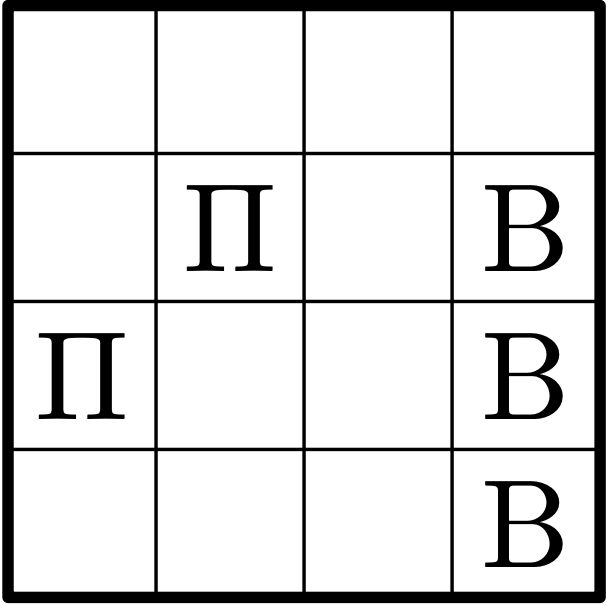
\includegraphics[width=0.1\textwidth]{table}\label{fig:table}
        \end{figure}

%21.9.7
        \item Вася записал в клетки таблицы $9 \times 9$ натуральные числа от 1 до 81 (в каждой клетке стоит по числу, все числа различны).
        Оказалось, что любые два числа, отличающихся на 3, стоят в соседних по стороне клетках.
        Верно ли, что обязательно найдутся две угловых клетки, разность чисел в которых делится на 6?

%21.9.9
        \item В алфавите $n > 1$ букв; словом является каждая конечная последовательность букв, в которой любые две соседние буквы различны.
        Слово называется хорошим, если из него нельзя вычеркнуть все буквы, кроме четырёх, так, чтобы осталась последовательность вида $aabb$, где $a$ и $b$ — различные буквы.
        Найдите наибольшее возможное количество букв в хорошем слове.

%20.9.1
        \item Изначально на столе лежали 10 куч конфет, в которых было $1, 2, \dotsc, 10$ конфет соответственно.
        Малыш решил перераспределить конфеты.
        На каждой нечётной минуте он выбирает одну из куч и делит её на две кучи, в каждой из которых хотя бы по одной конфете.
        На каждой чётной минуте он выбирает две кучи и объединяет их в одну (таким образом, первым действием он делит кучу на две).
        Может ли в некоторый момент оказаться, что все кучи на столе содержат одно и то же количество конфет?

%20.9.3
        \item  Коля и Дима играют в игру на доске $8 \times 8$, делая ходы по очереди, начинает Дима.
        Коля рисует в клетках крестики, а Дима накрывает прямоугольниками $1 \times 2$ (доминошками) пары соседних по стороне клеток доски.
        За свой ход Коля должен поставить один крестик в любую пустую клетку (т.е. в клетку, в которой ещё не нарисован крестик и которая ещё не покрыта доминошкой).
        Дима за свой ход должен накрыть доминошкой две соседних клетки (ещё не накрытые другими доминошками), в которых суммарно чётное число крестиков (0 или 2).
        Проигрывает тот, кто не может сделать ход.
        Кто из игроков имеет выигрышную стратегию?

%20.9.7
        \item Зелёный хамелеон всегда говорит правду, а коричневый хамелеон врёт и после этого немедленно зеленеет.
        В компании из 2019 хамелеонов (зелёных и коричневых) каждый по очереди ответил на вопрос, сколько среди них сейчас зелёных.
        Ответами были числа $1, 2, 3, \dotsc, 2019$ (в некотором порядке, причём не обязательно в указанном выше).
        Какое наибольшее число зелёных хамелеонов могло быть изначально?

%20.9.9
        \item Назовём многоугольник хорошим, если у него найдётся пара параллельных сторон.
        Некоторый правильный многоугольник разрезали непересекающимися (по внутренним точкам) диагоналями на несколько многоугольников так, что у всех этих многоугольников одно и то же нечётное количество сторон.
        Может ли оказаться, что среди этих многоугольников есть хотя бы один хороший?

    \end{enumerate_boxed}
\end{document}